\begin{exercise}{
    Consider the following abstract domain $Sign_k$ of $\left<\wp(\Z), \subseteq\right>$ where $k \in \Z$ is any given integer:
    \begin{center}
        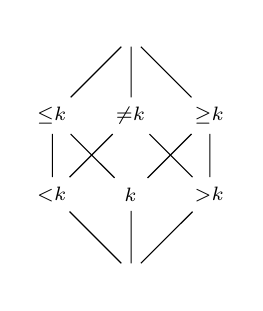
\begin{tikzpicture}
            \node (top) at (1, 3) {$\Z$};
            \node (leq) at (0, 2) {$\Z_{\leq k}$};
            \node (neq) at (1, 2) {$\Z_{\neq k}$};
            \node (geq) at (2, 2) {$\Z_{\geq k}$};
            \node (lt) at (0, 1) {$\Z_{< k}$};
            \node (eq) at (1, 1) {$\Z_{k}$};
            \node (gt) at (2, 1) {$\Z_{> k}$};
            \node (bot) at (1, 0) {$\varnothing$};

            \draw (top) -- (leq) -- (eq);
            \draw (top) -- (neq) -- (lt);
            \draw (top) -- (geq) -- (gt);
            \draw (leq) -- (lt) -- (bot);
            \draw (neq) -- (gt) -- (bot);
            \draw (geq) -- (eq) -- (bot);
        \end{tikzpicture}
    \end{center}
    Hence, $Sign_k$ is a parametric abstract domain of signs, where the constant 0 is replaced by any integer parameter $k \in \Z$. Provide sound definitions for the following abstract transfer functions: $\Bsharp{x \leq k}$, $\Asharp{x * y}$, $\Asharp{x / k}$, $\Asharp{x - y}$, which are as precise as possible, ideally the best correct approximation.
}
    \begin{align*}
        \Bsharp{x \leq k} s^\sharp &= \begin{cases}
            \bot^\sharp & \text{if } \Asharp{x} s^\sharp \in \{ \varnothing, \Z_{>k} \} \\
            s^\sharp [x \to \Z_{\leq k}] & \text{if } \Asharp{x} s^\sharp \in \{ \Z, \Z_{\leq k} \} \\
            s^\sharp [x \to \Z_k] & \text{if } \Asharp{x} s^\sharp \in \{ \Z_k, \Z_{\geq k} \} \\
            s^\sharp [x \to \Z_{< k}] & \text{if } \Asharp{x} s^\sharp \in \{ \Z_{< k}, \Z_{\neq k} \}
        \end{cases} \\
        \Asharp{x * y} s^\sharp &= \begin{cases}
            \varnothing & \text{if } \Asharp{x} s^\sharp = \varnothing \text{ or } \Asharp{y} s^\sharp = \varnothing \\
            \Z_k & \text{if } k = 0 \text{ and } (\Asharp{x} = \Z_k \text{ or } \Asharp{y} = \Z_k) \\
            \Asharp{y} s^\sharp & \text{if } k = 1 \text{ and } \Asharp{x} s^\sharp = \Z_k \\
            \Asharp{x} s^\sharp & \text{if } k = 1 \text{ and } \Asharp{y} s^\sharp = \Z_k \\
            ... \\
            \Z & \text{otherwise}
        \end{cases} \\
        \Asharp{x / k} s^\sharp &= \begin{cases}
            \varnothing & \text{if } \Asharp{x} s^\sharp = \varnothing \text{ or } k = 0 \\
            \Asharp{x} s^\sharp & \text{if } k = 1 \\
            \Z_{< k} & \text{if } k > 1 \text{ and } \Asharp{x} s^\sharp \in \{ \Z_{< k}, \Z_{\leq k} \} \\
            \Z_{> k} & \text{if } k < 0 \text{ and } \Asharp{x} s^\sharp \in \{ \Z_{< k}, \Z_{\leq k} \} \\
            \Z_{\neq k} & \text{if } \Asharp{x} = \Z_k \\
            ... \\
            \Z & \text{otherwise}
        \end{cases} \\
        \Asharp{x - y} s^\sharp &= \begin{cases}
            \varnothing & \text{if } \Asharp{x} s^\sharp = \varnothing \text{ or } \Asharp{y} s^\sharp = \varnothing \\
            \Asharp{x} s^\sharp & \text{if } k = 0 \text{ and } \Asharp{y} s^\sharp = \Z_k \\
            \Asharp{-y} s^\sharp & k = 0 \text{ and } \Asharp{x} s^\sharp = Z_k \\
            \Z_{< k} & \text{if } k > 0, \Asharp{x} \in \{ \Z_{< k}, \Z_{\leq k}, Z_k \} \text{ and } \Asharp{y} \in \{ \Z_{> k}, \Z_{\geq k}, Z_k \} \\
            \Z_{> k} & \text{if } k < 0, \Asharp{x} \in \{ \Z_{> k}, \Z_{\geq k}, Z_k \} \text{ and } \Asharp{y} \in \{ \Z_{< k}, \Z_{\leq k}, Z_k \} \\
            ... \\
            \Z & \text{otherwise}
        \end{cases} \\
    \end{align*}
\end{exercise}
